\documentclass[12pt]{beamer}

\usepackage[italian]{babel}
\usepackage{csquotes}
\usepackage{dirtytalk}
\usepackage{fancyvrb}
\usepackage{graphicx}
\usepackage[utf8]{inputenc}
\usepackage{minted}
\usepackage{soul}
\usepackage{subcaption}
\usepackage{tikz}

\usetheme{Copenhagen}
\setbeamertemplate{navigation symbols}{}
\setbeamertemplate{bibliography entry title}{}
\setbeamertemplate{bibliography entry location}{}
\setbeamertemplate{bibliography entry note}{}

\usetikzlibrary{shapes}

\newtheorem{definizione}{Definizione}

\title{
  Ho sconfitto gli emendamenti\\
  di Calderoli con un software
}
\author{Jacopo Notarstefano}
\date{29 maggio 2016}

\begin{document}
  \begin{frame}[plain]
    \titlepage{}
  \end{frame}

  \begin{frame}{\texttt{\$ whoami}}
    Mi chiamo Jacopo Notarstefano e sono Junior Fellow al CERN\@. In particolare
    lavoro a INSPIRE, un motore di ricerca per articoli, preprint e dati
    nell'ambito della fisica delle alte energie.

    \vspace{0.5cm}

    Il mio Twitter è \textbf{@Jaconotar} e i miei DM sono aperti per domande,
    commenti e chiarimenti. Ask Me Anything (AMA)!
  \end{frame}

  \begin{frame}{Un chiarimento importante}
    Il CERN non ha niente a che vedere con ciò di cui parlerò oggi.

    \vspace{0.5cm}

    Il codice di cui parlerò è stato sviluppato nel mio tempo libero, le
    opinioni che esprimerò sono personali e non riflettono necessariamente
    quelle dei miei colleghi, superiori o del CERN.
  \end{frame}

  \begin{frame}{Article spinning}
    Aziende e privati competono in ogni modo per raggiungere le prime posizioni
    nei risultati di Google per certe keyword.

    \vspace{0.5cm}

    L'\textbf{article spinning} è una tecnica ormai in disuso per ottenere
    questo obiettivo. A partire da una pagina base ne vengono generate un numero
    elevato di variazioni: ciascuna di queste linka una pagina di cui si
    desidera migliorare il posizionamento.
  \end{frame}

  \begin{frame}[fragile]
    \frametitle{Spintax}

    La generazione di queste pagine avviene usando un'opportuna sintassi,
    talvolta detta \textbf{spintax}. Ad esempio

    \begin{semiverbatim}
\{Ciao|Salve\}, questa è \{spin syntax|spintax\}.
\end{semiverbatim}

    genera

    \begin{figure}
      \centering
      \begin{tikzpicture}
        \draw (   0, 0) rectangle (   2, 2) node[midway,align=center,font=\scriptsize] {Ciao, questa\\ è spin syntax};
        \draw ( 2.5, 0) rectangle ( 4.5, 2) node[midway,align=center,font=\scriptsize] {Ciao, questa\\ è spintax};
        \draw (   5, 0) rectangle (   7, 2) node[midway,align=center,font=\scriptsize] {Salve, questa\\ è spin syntax};
        \draw ( 7.5, 0) rectangle ( 9.5, 2) node[midway,align=center,font=\scriptsize] {Salve, questa\\ è spintax};
      \end{tikzpicture}
    \end{figure}
\end{frame}

  \begin{frame}{La ``fine'' dell'article spinning}
    \begin{figure}
      \centering
      \begin{subfigure}[b]{0.45\textwidth}
        \centering
        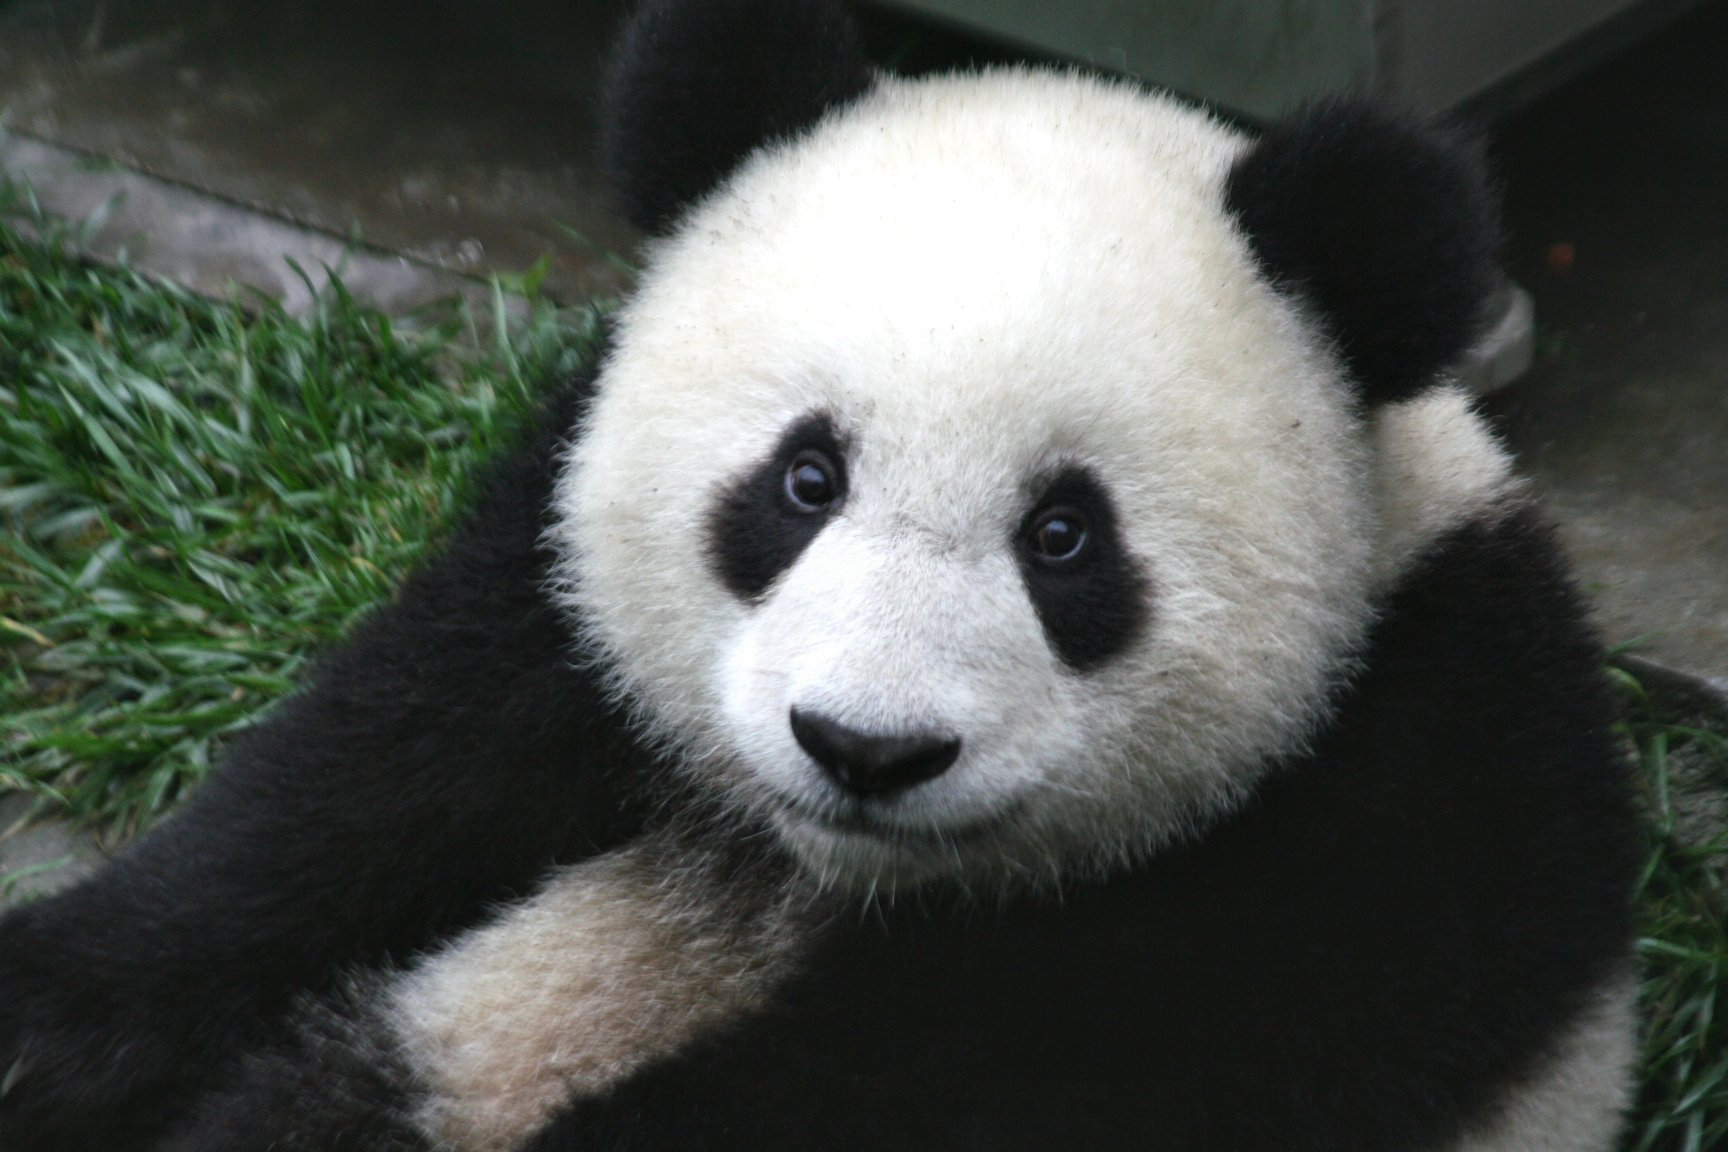
\includegraphics[width=\textwidth]{tex/img/panda}
      \end{subfigure}
      \hspace{0.05\textwidth}
      \begin{subfigure}[b]{0.45\textwidth}
        \centering
        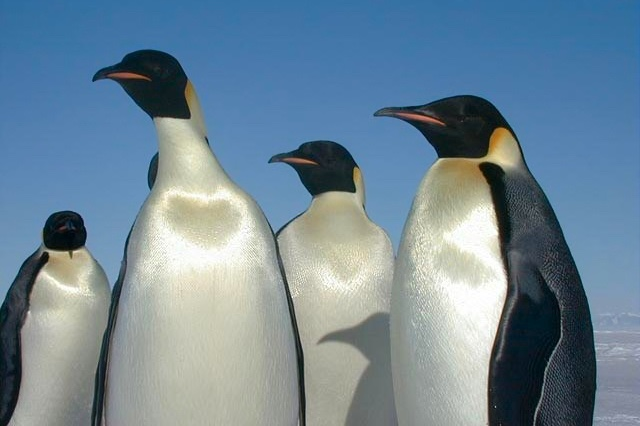
\includegraphics[width=\textwidth]{tex/img/penguins}
      \end{subfigure}
    \end{figure}

    A partire dal 2010 una serie di aggiornamenti di Google chiamati ``Panda'' e
    ``Penguin'' ha cominciato a penalizzare fortemente i siti contenenti testi
    duplicati.
  \end{frame}

  \begin{frame}{Calderoli, 1/3}
    \begin{figure}
      \centering
      \fbox{
\includegraphics[width=\textwidth]{tex/img/calderoli1}}
    \end{figure}

    I senatori Calderoli e Crosio trovano una nuova applicazione dell'article
    spinning: la generazione di grandi quantità di emendamenti a scopo
    ostruzionistico.
  \end{frame}

  \begin{frame}{Calderoli, 2/3}
    \begin{figure}
      \centering
      \fbox{
\includegraphics[width=\textwidth]{tex/img/calderoli2}}
    \end{figure}

    La prima applicazione di questa tecnica ostruzionistica ottiene un successo
    parziale: la legge passerà, ma verranno rinegoziati alcuni articoli e
    slitteranno alcuni tempi tenici.
  \end{frame}

  \begin{frame}{Calderoli, 3/3}
    \begin{figure}
      \centering
      \fbox{
\includegraphics[width=\textwidth]{tex/img/calderoli3}}
    \end{figure}

    È più complicato valutare il successo della seconda applicazione, visto il
    peculiare clima politico che si è creato intorno all'emendamento Marcucci.
  \end{frame}

  \begin{frame}[fragile]
    \frametitle{Il caso del DDL Cirinnà, 1/3}

    Andiamo a vedere che aspetto hanno due emendamenti generati in questo modo.

    \vspace{0.25cm}

    \fontsize{2pt}{3}
    \textbf{1.450}
    \begin{semiverbatim}Sostituire il comma 1 con il seguente:

  "1. In osservanza del principio costituzionale di cui agli articoli 29 e 31
      della Costituzione, ai sensi della lettera m) secondo comma ex art. 117 della
      Costituzione, la presente legge tutela e garantisce il ruolo sociale
      dell'educazione dei figli attraverso il riconoscimento delle figure
      genitoriali quali madre e padre."

Conseguentemente, sopprimere gli articoli da 2 a 10 e all'articolo 11 sopprimere
le parole: "o da un'unione civile".
\end{semiverbatim}

    \fontsize{2pt}{3}
    \textbf{1.451}
    \begin{semiverbatim}Sostituire il comma 1 con il seguente:

  "1. In osservanza del principio costituzionale di cui agli articoli 29 e 31
      della Costituzione, ai sensi della lettera m) secondo comma ex art. 117 della
      Costituzione, la presente legge tutela e garantisce il ruolo sociale
      dell'educazione dei figli attraverso il riconoscimento delle figure
      genitoriali quali madre e padre."

Conseguentemente, sopprimere gli articoli da 2 a 10.
\end{semiverbatim}
\end{frame}

  \begin{frame}[fragile]
    \frametitle{Il caso del DDL Cirinnà, 2/3}

    I due precedenti emendamenti differiscono soltanto per l'aggiunta di una
    frase finale. Il successivo aggiunge un ulteriore paragrafo.

    \vspace{0.25cm}

    \fontsize{2pt}{3}
    \textbf{1.452}
    \begin{semiverbatim}Sostituire il comma 1 con il seguente:

  "1. In osservanza del principio costituzionale di cui agli articoli 29 e 31
      della Costituzione, ai sensi della lettera m) secondo comma ex art. 117
      della Costituzione, la presente legge tutela e garantisce il ruolo sociale
      dell'educazione dei figli attraverso il riconoscimento delle figure
      genitoriali quali madre e padre."

Conseguentemente, sopprimere gli articoli da 2 a 10 e all'articolo 11 sopprimere
le parole: "o da un'unione civile".

Conseguentemente, dopo l'articolo, aggiungere il seguente:

  "Art. 23-bis. (Disciplina transitoria)

  1. La presente legge entra in vigore dopo l'approvazione di una legge
     costituzionale, adottata ai sensi dell'articolo 138 della Costituzione, di
     modifica degli articoli 29, 30 e 31 della Costituzione."
\end{semiverbatim}
\end{frame}

  \begin{frame}[fragile]
    \frametitle{Il caso del DDL Cirinnà, 3/3}

    Non è difficile ricostruire la spintax che potrebbe aver generato i
    precedenti tre emendamenti.

    \vspace{0.25cm}

    \fontsize{2pt}{3}
    \begin{semiverbatim}Sostituire il comma 1 con il seguente:

  "1. In osservanza del principio costituzionale di cui agli articoli 29 e 31
      della Costituzione, ai sensi della lettera m) secondo comma ex art. 117
      della Costituzione, la presente legge tutela e garantisce il ruolo sociale
      dell’educazione dei figli attraverso il riconoscimento delle figure
      genitoriali quali madre e padre."

Conseguentemente, sopprimere gli articoli da 2 a 10\{| e all'articolo 11
sopprimere le parole "o da un'unione civile"\}.
\{|
Conseguentemente, dopo l'articolo, aggiungere il seguente:

  "Art. 23-bis. (Disciplina transitoria)

  1. La presente legge entra in vigore dopo l'approvazione di una legge
     costituzionale, adottata ai sensi dell'articolo 138 della Costituzione, di
     modifica degli articoli 29, 30 e 31 della Costituzione."\}
\end{semiverbatim}
\end{frame}

  \begin{frame}{Gli Open Data del Senato}
    Il sito del Senato offre una grande varietà di dati su leggi, iter
    legislativi e attività dei Senatori in formati liberi (CSV, XML, JSON,
    \textellipsis) e in modo facile da interrogare (SPARQL).

    \vspace{0.5cm}

    La qualità di dati e metadati è ottima, la documentazione è scarna ma
    chiara.
  \end{frame}

  \begin{frame}{Un piccolo intoppo}
    Purtroppo l'endpoint SPARQL non offre i testi degli emendamenti, quindi
    siamo costretti a scrivere uno spider per scaricarli dal sito del Senato.

    \vspace{0.25cm}

    \inputminted[fontsize=\tiny]{python}{tex/src/spider.py}
  \end{frame}

  \begin{frame}{Hierarchical Clustering: il problema}
    Vogliamo raggruppare un certo numero di oggetti in un numero ignoto di
    partizioni, detti \textbf{cluster}, in modo che oggetti vicini appartengano
    allo stesso cluster.

    \vspace{0.25cm}

    \begin{figure}
      \centering
      \begin{tikzpicture}
        \node [draw,circle] (A) at (-6, 1) {A};
        \node [draw,circle] (B) at (-4, 2) {B};
        \node [draw,circle] (C) at (-0.5, 2) {C};
        \node [draw,circle] (D) at (0.5, 3) {D};
        \node [draw,circle] (E) at (2, 2) {E};

        \draw[->, -latex] (-7.5, 0.5) -- (2.5, 0.5);
        \draw[->, -latex] (-7, 0) -- (-7, 4.5);

        \path[use as bounding box] (-1,-1) rectangle (10,4);
      \end{tikzpicture}
    \end{figure}
  \end{frame}

  \begin{frame}{Hierarchical Clustering: l'idea}
    L'idea più semplice che ci viene in mente è fondere insieme i due nodi più
    vicini e ripetere il procedimento, fino a che non arriviamo a un unico
    cluster.

    \vspace{0.25cm}

    \begin{figure}
      \centering
      \begin{tikzpicture}
        \node [draw,circle] (A) at (-6, 1) {A};
        \node [draw,circle] (B) at (-4, 2) {B};
        \node [draw,ellipse,rotate=45,minimum width=2cm] (CD) at (0, 2.5) {CD};
        \node [draw,circle] (E) at (2, 2) {E};

        \draw[->, -latex] (-7.5, 0.5) -- (2.5, 0.5);
        \draw[->, -latex] (-7, 0) -- (-7, 4.5);

        \path[use as bounding box] (-1,-1) rectangle (10,4);
      \end{tikzpicture}
    \end{figure}
  \end{frame}

  \begin{frame}{Hierarchical Clustering: l'albero delle fusioni, 1/3}
    \begin{figure}
      \centering
      \begin{tikzpicture}[sloped]
        \node (A) at (-6,0) {A};
        \node (B) at (-4,0) {B};
        \node (C) at (-0.5,0) {C};
        \node (D) at (0.5,0) {D};
        \node (E) at (2,0) {E};

        \node (CD) at (0,1) {};
        \node (CDE) at (1,2) {};

        \draw (C) |- (CD.center);
        \draw (D) |- (CD.center);

        \draw [dashed] (E) |- (CDE.center);
        \draw [dashed] (CD.center) |- (CDE.center);

        \draw [dotted] (-7,1) -- (CD);
        \node [left] (dCD) at (-7,1) {\small \(d(C,D)\)};

        \draw[->,-latex] (-7,0) -- node[above]{distanza} (-7,6);
      \end{tikzpicture}
    \end{figure}
  \end{frame}

  \begin{frame}{Hierarchical Clustering: l'albero delle fusioni, 2/3}
    \begin{figure}
      \centering
      \begin{tikzpicture}[sloped]
        \node (A) at (-6,0) {A};
        \node (B) at (-4,0) {B};
        \node (C) at (-0.5,0) {C};
        \node (D) at (0.5,0) {D};
        \node (E) at (2,0) {E};

        \node (AB) at (-4.5,3) {};
        \node (CD) at (0,1) {};
        \node (CDE) at (1,2) {};
        \node (ABCDE) at (-1.5,5) {};

        \draw  (A) |- (AB.center);
        \draw  (B) |- (AB.center);
        \draw  (C) |- (CD.center);
        \draw  (D) |- (CD.center);
        \draw  (E) |- (CDE.center);
        \draw  (CD.center) |- (CDE.center);
        \draw  (AB.center) |- (ABCDE.center);
        \draw  (CDE.center) |- (ABCDE.center);

        \draw[->,-latex] (-7,0) -- node[above]{distanza} (-7,6);
      \end{tikzpicture}
    \end{figure}
  \end{frame}

  \begin{frame}{Hierarchical Clustering: l'albero delle fusioni, 3/3}
    \begin{figure}
      \centering
      \begin{tikzpicture}[sloped]
        \node (A) at (-6,0) {A};
        \node (B) at (-4,0) {B};
        \node (C) at (-0.5,0) {C};
        \node (D) at (0.5,0) {D};
        \node (E) at (2,0) {E};

        \node (AB) at (-4.5,3) {};
        \node (CD) at (0,1) {};
        \node (CDE) at (1,2) {};
        \node (ABCDE) at (-1.5,5) {};

        \draw  (A) |- (AB.center);
        \draw  (B) |- (AB.center);
        \draw  (C) |- (CD.center);
        \draw  (D) |- (CD.center);
        \draw  (E) |- (CDE.center);
        \draw  (CD.center) |- (CDE.center);
        \draw  (AB.center) |- (ABCDE.center);
        \draw  (CDE.center) |- (ABCDE.center);

        \draw [thick,red] (-7.5,1.5) -- (2.5,1.5);
        \draw [thick,blue] (-7.5,4.5) -- (2.5,4.5);

        \draw[->,-latex] (-7,0) -- node[above]{distanza} (-7,6);
      \end{tikzpicture}
    \end{figure}
  \end{frame}

  \begin{frame}{La Distanza di Jaccard: l'idea, 1/2}
    La vicinanza semantica di due testi può essere dedotta dalla vicinanza
    sintattica delle \emph{parole} dei due testi. Ad esempio:

    \vspace{0.25cm}

    \begin{itemize}
      \item Oggi sono andato al mercato con mia mamma.
      \item Io e mia mamma oggi ci siamo recati al mercato.
      \item Meglio viaggiare in treno che viaggiare in macchina.
    \end{itemize}
  \end{frame}

  \begin{frame}{La Distanza di Jaccard: l'idea, 2/2}
    La vicinanza semantica di due testi può essere dedotta dalla vicinanza
    sintattica delle \emph{parole} dei due testi. Ad esempio:

    \vspace{0.25cm}

    \begin{itemize}
      \item \textbf{Oggi} sono andato \textbf{al mercato} con \textbf{mia mamma}.
      \item Io e \textbf{mia mamma oggi} ci siamo recati \textbf{al mercato}.
      \item Meglio viaggiare in treno che viaggiare in macchina.
    \end{itemize}
  \end{frame}

  \begin{frame}{La Distanza di Jaccard: la definizione}
    \begin{definizione}[Distanza di Jaccard]
      Siano \(A\) e \(B\) due documenti, e sia \(\text{\texttt{token}}(X)\) la
      funzione che ritorna l'insieme delle parole distinte del documento \(X\).

      \vspace{0.25cm}

      Allora chiamiamo \textbf{Distanza di Jaccard} la seguente funzione:
      \[
        d_{\text{Jaccard}}(A, B) = 1 - \frac
          {\left|\text{\texttt{token}}(A)\cap\text{\texttt{token}}(B)\right|}
          {\left|\text{\texttt{token}}(A)\cup\text{\texttt{token}}(B)\right|}
      \]
    \end{definizione}
  \end{frame}

  \begin{frame}{L'albero delle fusioni dei primi cento emendamenti}
    \begin{figure}
      \centering
      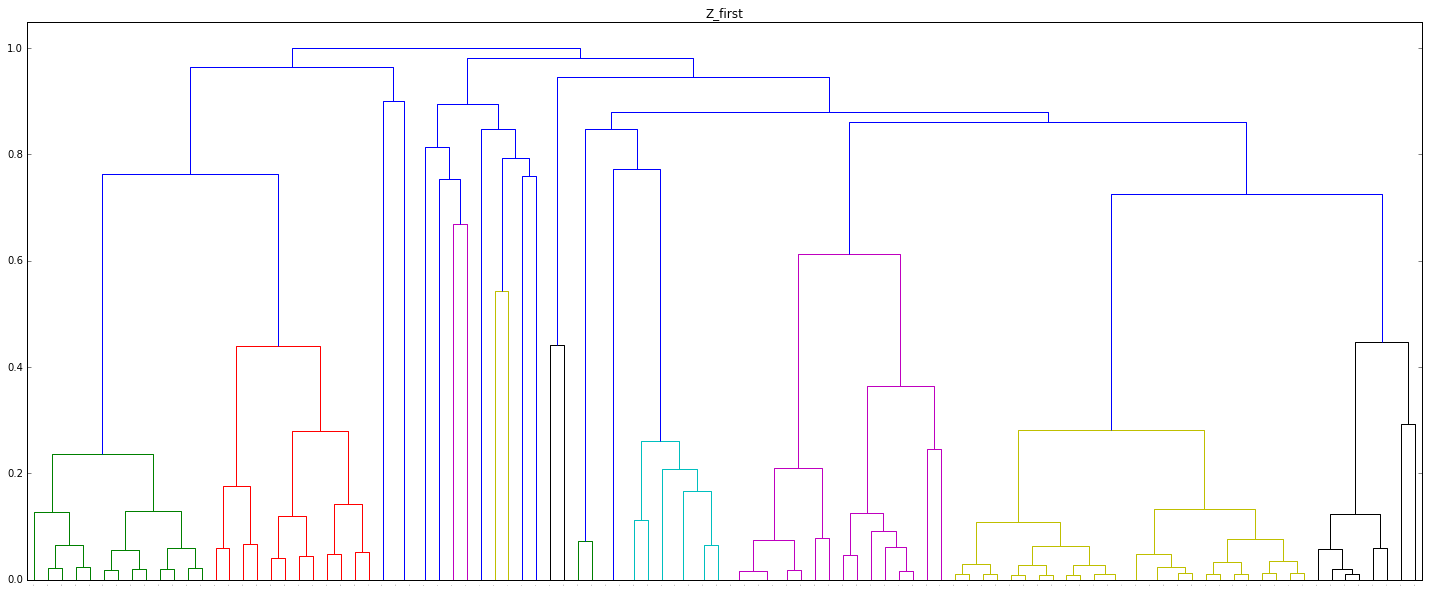
\includegraphics[width=\textwidth]{tex/img/tree-first}
    \end{figure}

    \vspace{0.25cm}

    Una volta definita una distanza fra emendamenti possiamo applicare HC\@.
    Per verificare il buon funzionamento proviamo ad applicarlo ai primi cento
    emendamenti.
  \end{frame}

  \begin{frame}{Un cluster di emendamenti}
    \begin{figure}
      \centering
      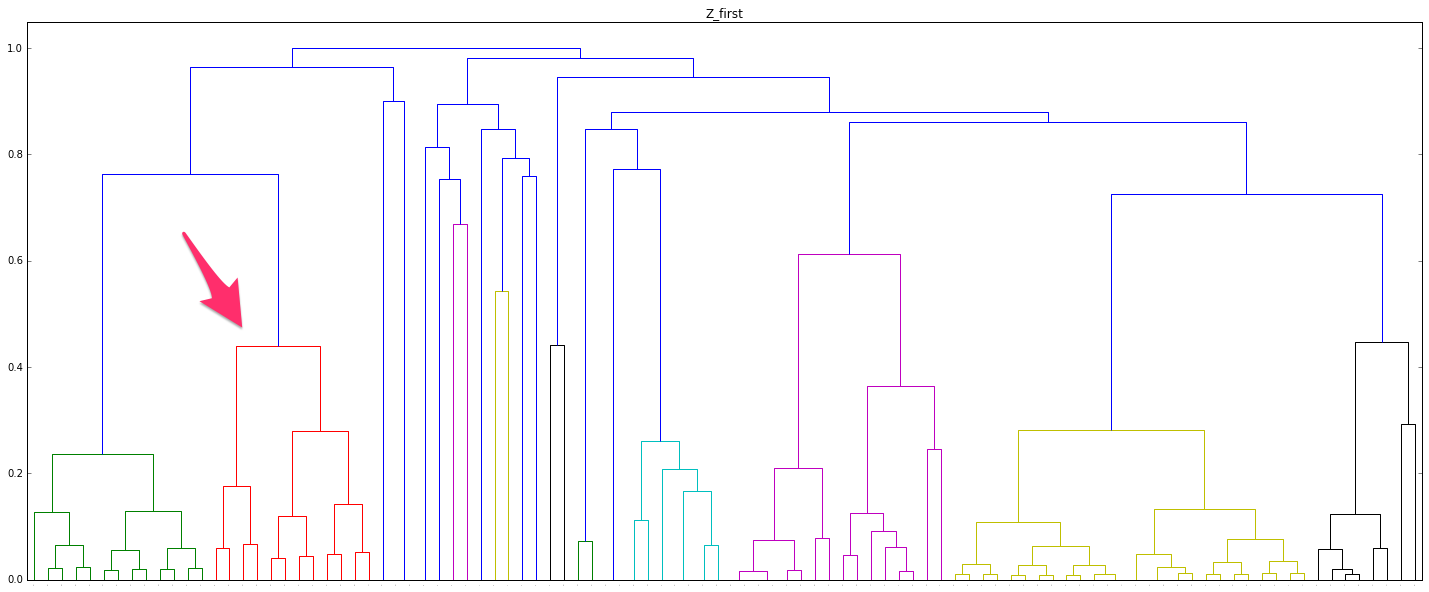
\includegraphics[width=\textwidth]{tex/img/tree-first-first-cluster}
    \end{figure}

    \vspace{0.25cm}

    {
      \scriptsize
      \textbf{1.2511}: Sopprimere gli articoli 1, 2, 3, 4, 5, 6, 7, 8, 9, 10, 11.

      \textbf{1.2510}: Sopprimere gli articoli 1, 2, 3, 4, 5, 6, 7, 8, 9, 10, 11, 12.

      \textbf{1.2509}: Sopprimere gli articoli 1, 2, 3, 4, 5, 6, 7, 8, 9, 10, 11, 12, 13.

    }
  \end{frame}

  \begin{frame}{Un altro cluster di emendamenti}
    \begin{figure}
      \centering
      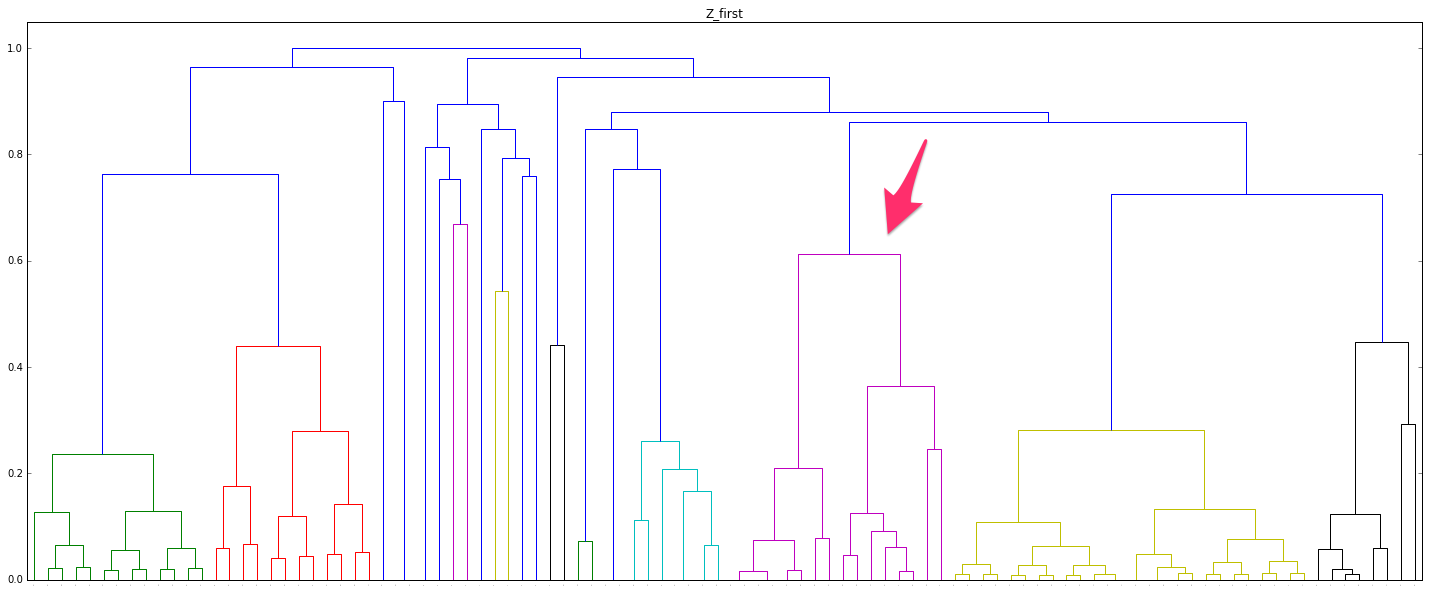
\includegraphics[width=\textwidth]{tex/img/tree-first-second-cluster}
    \end{figure}

    \vspace{0.25cm}

    {
      \scriptsize
      \textbf{01.8007}: All'articolo, premettere il seguente: «Art. 01. (Società economiche volte\textellipsis

      \textbf{01.8006}: All'articolo, premettere il seguente: «Art. 01. (Esclusività delle prerog\textellipsis

      \textbf{01.8002}: All'articolo, premettere il seguente: «Art. 01. (Esclusività della famigl\textellipsis

    }
  \end{frame}

  \begin{frame}{Emendamenti che non formano un cluster}
    \begin{figure}
      \centering
      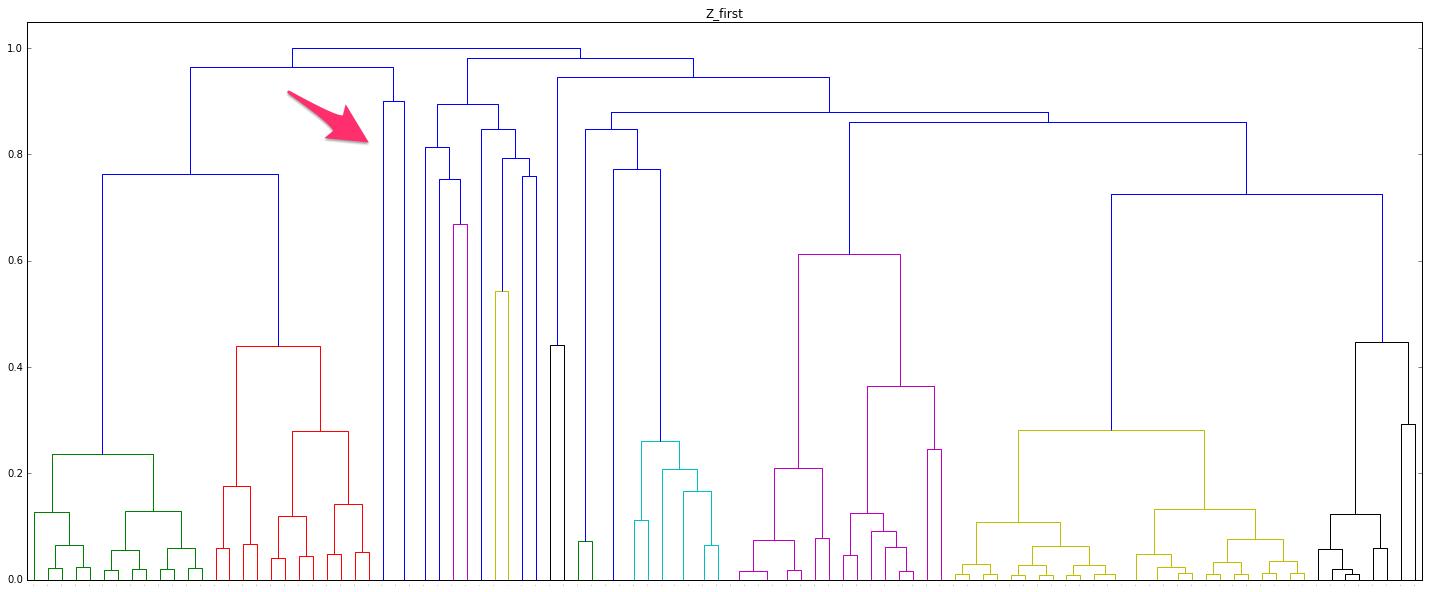
\includegraphics[width=\textwidth]{tex/img/tree-first-no-cluster}
    \end{figure}

    \vspace{0.25cm}

    È interessante notare che le questioni pregiudiziali, tutte diverse fra
    loro, non paiono formare alcun cluster.
  \end{frame}

  \begin{frame}{L'albero delle fusioni di tutti gli emendamenti}
    \begin{figure}
      \centering
      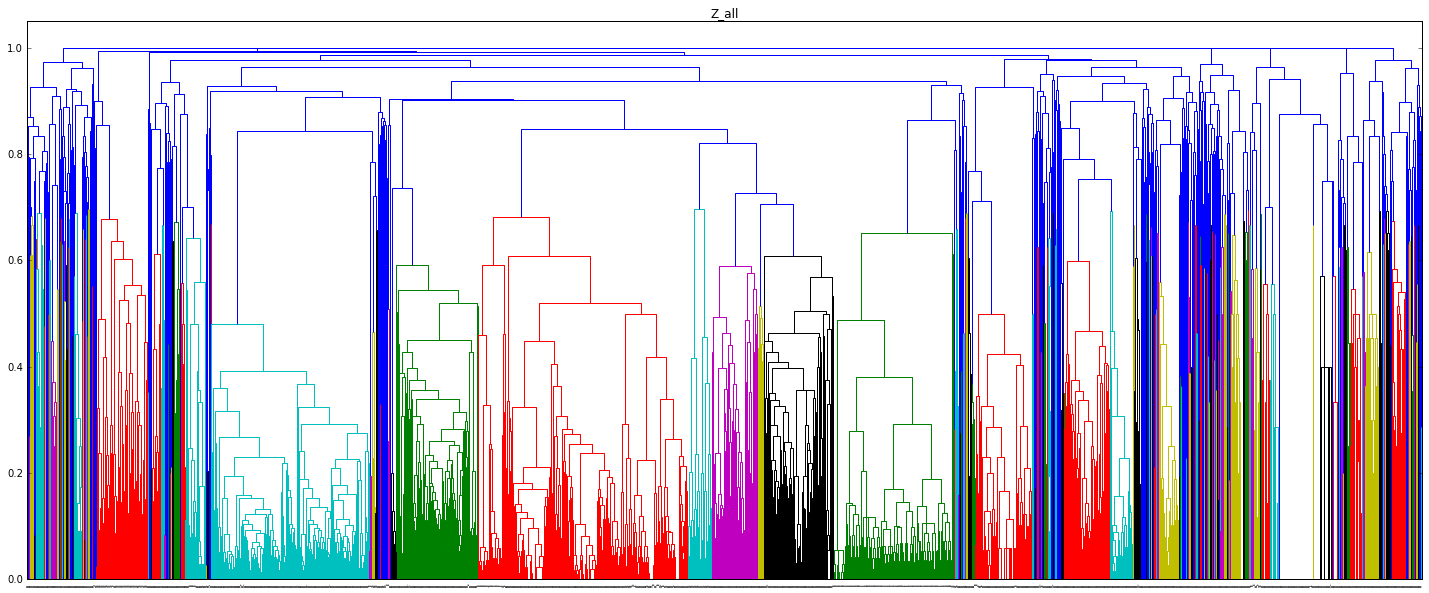
\includegraphics[width=\textwidth]{tex/img/tree-all}
    \end{figure}

    \vspace{0.25cm}

    In cinque minuti siamo in grado di far girare l'algoritmo su tutti gli
    emendamenti del DDL Cirinnà (\(\approx 5000)\).
  \end{frame}

  \begin{frame}{E poi?}
    Una volta raccolti generati i cluster abbiamo due alternative:

    \vspace{0.25cm}

    \begin{enumerate}
      \item Chi presiede il Senato può \mbox{invocare} il comma 8 dell'articolo 100
        del regolamento del Senato:
        \begin{displayquote}
          Il Presidente può stabilire, con decisione inappellabile, la
          inammissibilità di emendamenti privi di ogni reale portata
          modificativa (\textellipsis)
        \end{displayquote}
      \item Un altro parlamentare può depositare un piccolo emendamento
        ``canguro'' per ciascun cluster, riducendo drasticamente il numero di
        votazioni.
    \end{enumerate}
  \end{frame}

  \begin{frame}[plain]
    \titlepage{}
  \end{frame}

  \title[Ho sconfitto gli emendamenti di Calderoli con un software]{
    \st{Ho sconfitto} È possibile sconfiggere gli\\
    emendamenti di Calderoli con un software
  }
  \begin{frame}[plain]
    \titlepage{}
  \end{frame}

  \begin{frame}{Ringraziamenti}
    \begin{figure}
      \centering
      
\includegraphics[width=0.5\linewidth]{tex/img/folks}
    \end{figure}

    Grazie a tutti per l'attenzione e a Wired per avermi invitato.

    \vspace{0.25cm}

    Il mio Twitter è \textbf{@Jaconotar} e i miei DM sono aperti per domande,
    commenti e chiarimenti. Ask Me Anything (AMA)!
  \end{frame}
\end{document}
